Major phase boundaries in the Earth's mantle and core have been
identified with sharp transitions in the 
seismic wave velocities and the density distribution of the 
PREM model.

The depth distribution of the mineral composition for a pyrolitic mantle model
is shown in the following figure:

\begin{center}
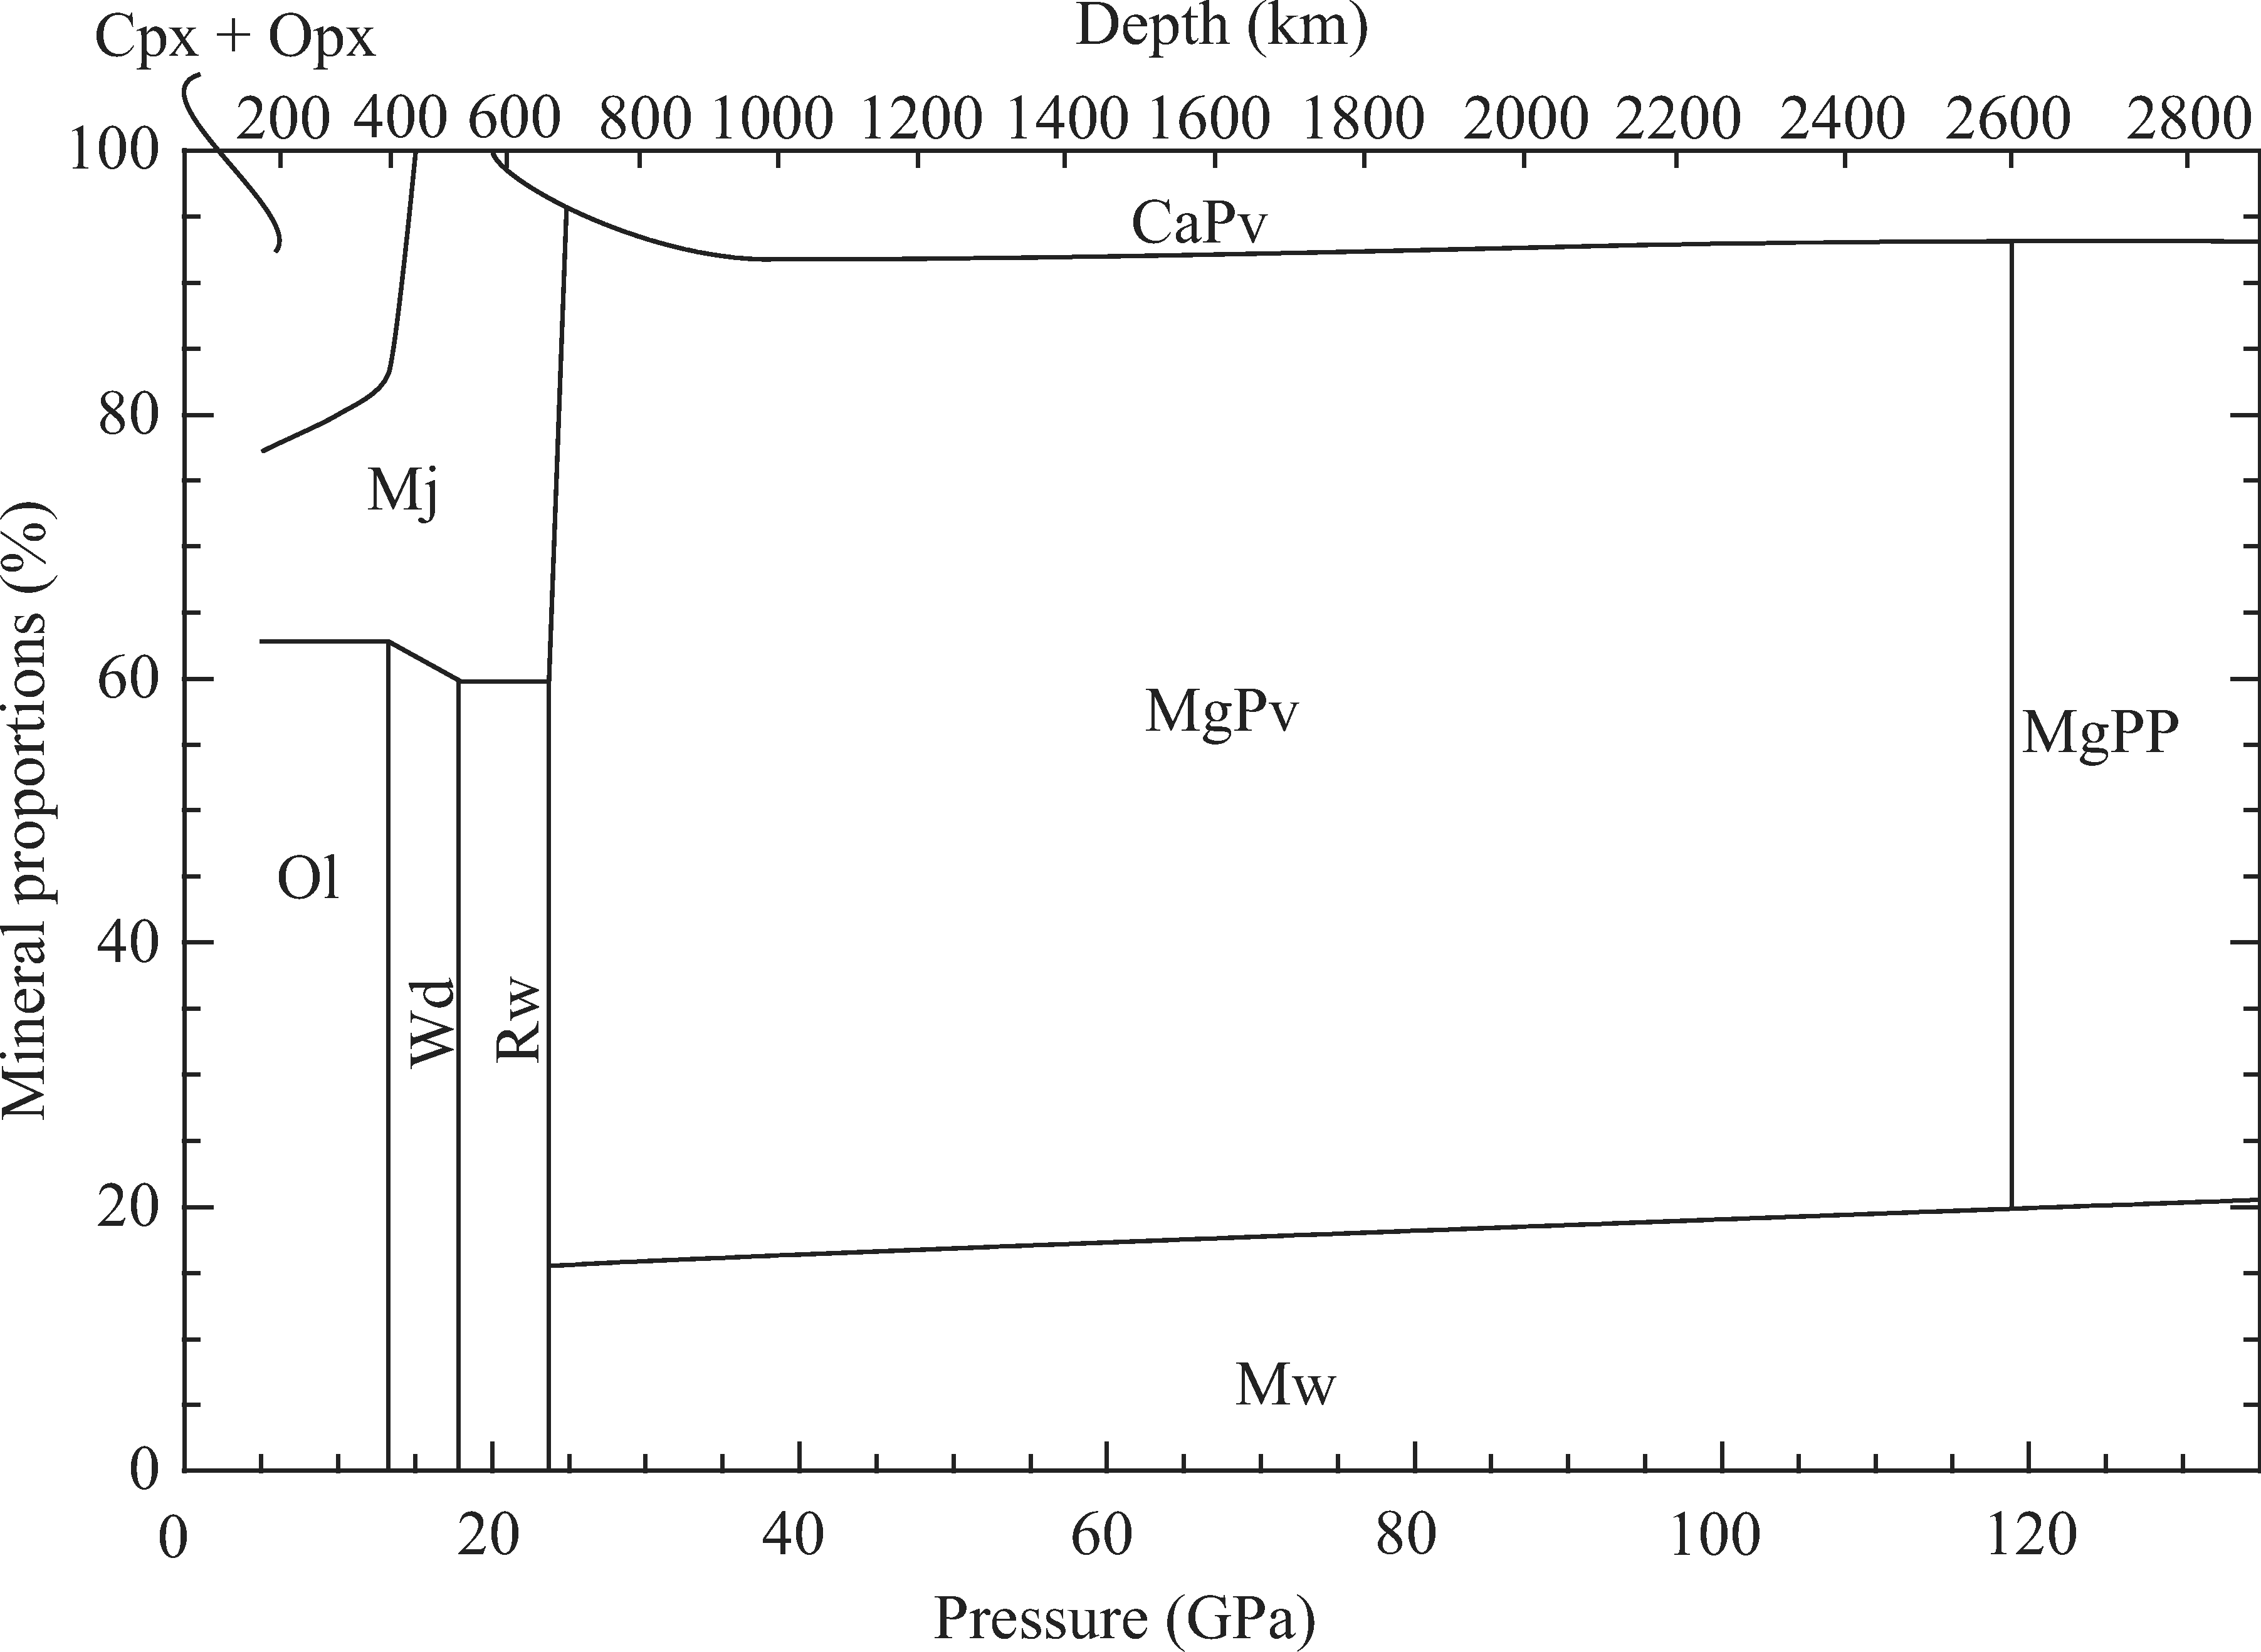
\includegraphics[width=10cm]{images/gravity/hirose_fig2}\\
{\captionfont
          Pressure/depth distribution of mineral assemblage for a pyrolitic
          mantle model.
          Cpx: clinopyroxene,
          Opx: orthopyroxene,
          Mj: majorite garnet,
          Ol: olivine,
          Wd: wadsleyite,
          Rw: ringwoodite,
          CaPv: $CaSiO_3$ perovskite
          MgPv: $MgSiO_3$-rich perovskite,
          MgPP: $MgSiO_3$-rich post-perovskite,
          Mw: magnesiow\"{u}stite.
(From: (Hirose, 2007))
}
\end{center}

This figure clearly illustrates the different mineral composition 
of the upper and lower mantle regions separated by the major
phase boundary near 660 km depth ($\sim$ 24 GPa),
where the ringwoodite polymorph of olivine, 
$\mathrm{(Mg,Fe)_2SiO_4}$,
transforms (dissociates) into a mineral assemblage of perovskite, 
$\mathrm{(Mg,Fe)SiO_3}$ and
magnesiow\"{u}stite, 
$\mathrm{(Mg,Fe)O}$.

For a given mantle composition, for instance for a pyrolitic mantle,
the pressure-temperature mineral phase diagram can be determined
for the relevant $P,T$ range of the Earth's mantle by HPT experiments
and mineral physics theory.
A sharp transition at a pressure $P_t$ in the PREM model can then be 
located at the corresponding pressure in the phase diagram by the 
intersection of the $P_t$ isobar with the diagram phase boundaries.
The (possibly multiple) intersection points define the corresponding
transition temperature $T_t$. 
The pressure-temperature point located in the phase diagram
defines an `anchor point' that constrains the geotherm.
In this procedure the phase transition is used as a mantle/core 
thermometer.

This way several $(P,T)$ `anchor points' of the geotherm have
been determined, related to the solid state phase transition near 
660 km depth and the solid/liquid inner/outer core boundary at 
1220 km from the Earth's centre.

The following figure from Boehler (1996) \cite{boeh96})
illustrates the determination of anchor points of the geotherm at the 
phase boundary near 660 km depth
($P_{660}=24 \mathrm{GPa}, T_{660}=1900 \pm 100$ K)
and at the boundary between the outer and inner core at 5150 km depth,
($P_{ICB}=330 \mathrm{GPa}, T_{ICB}=4850 \pm 200$ K).

\begin{center}
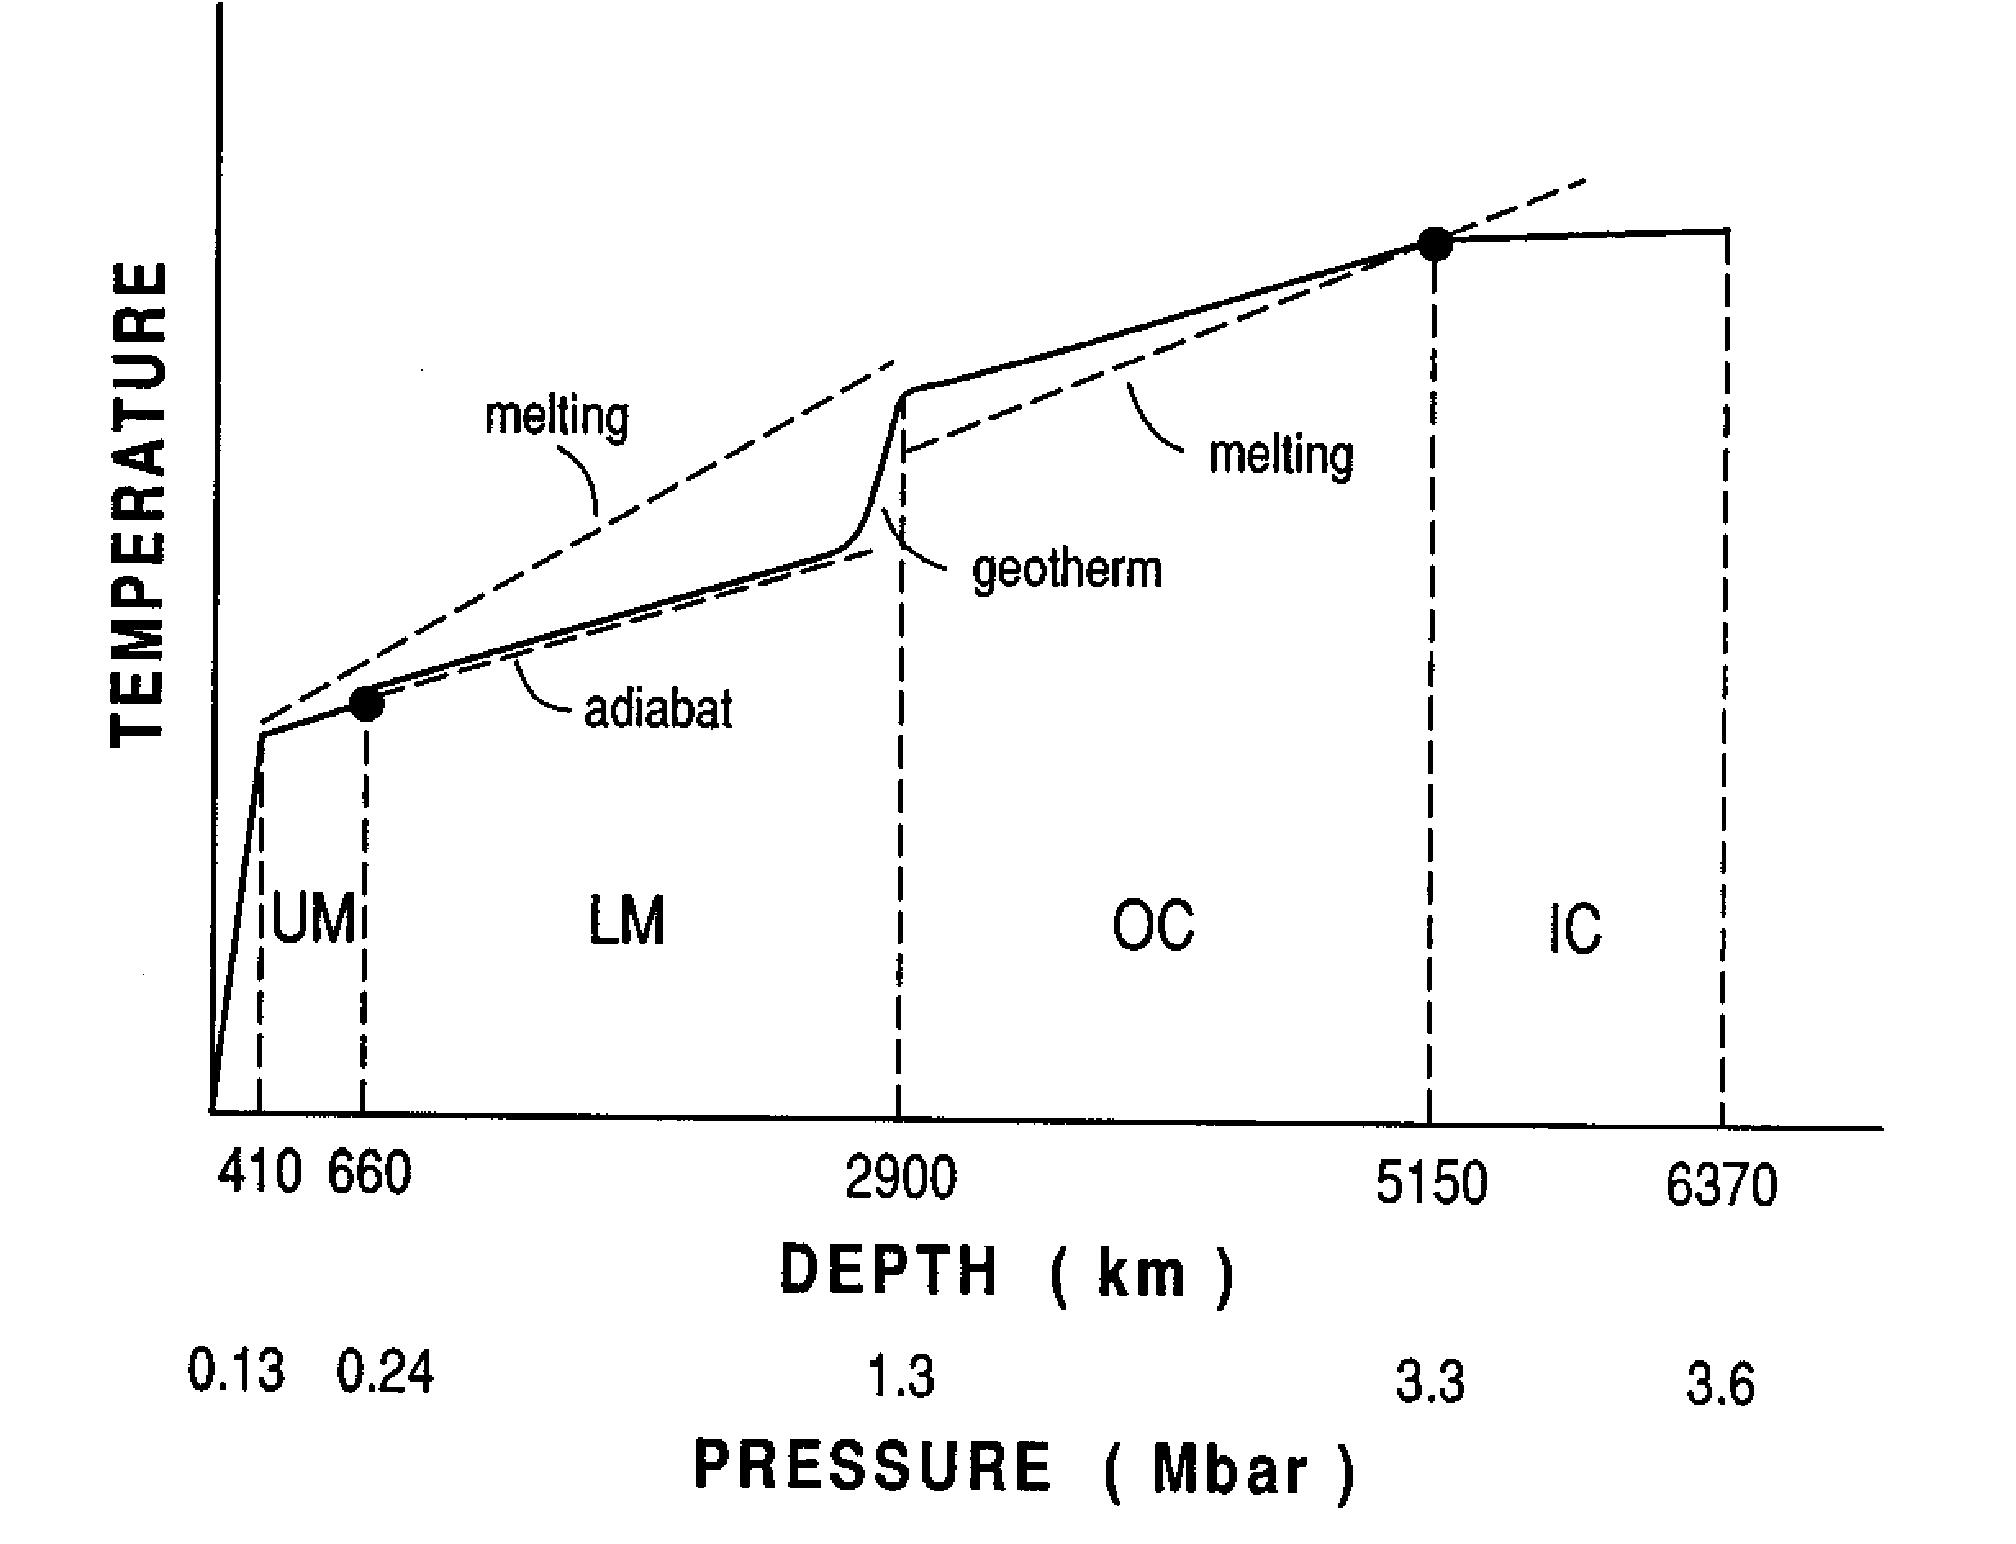
\includegraphics[width=7cm]{images/gravity/boehler_annrev96_fig1}
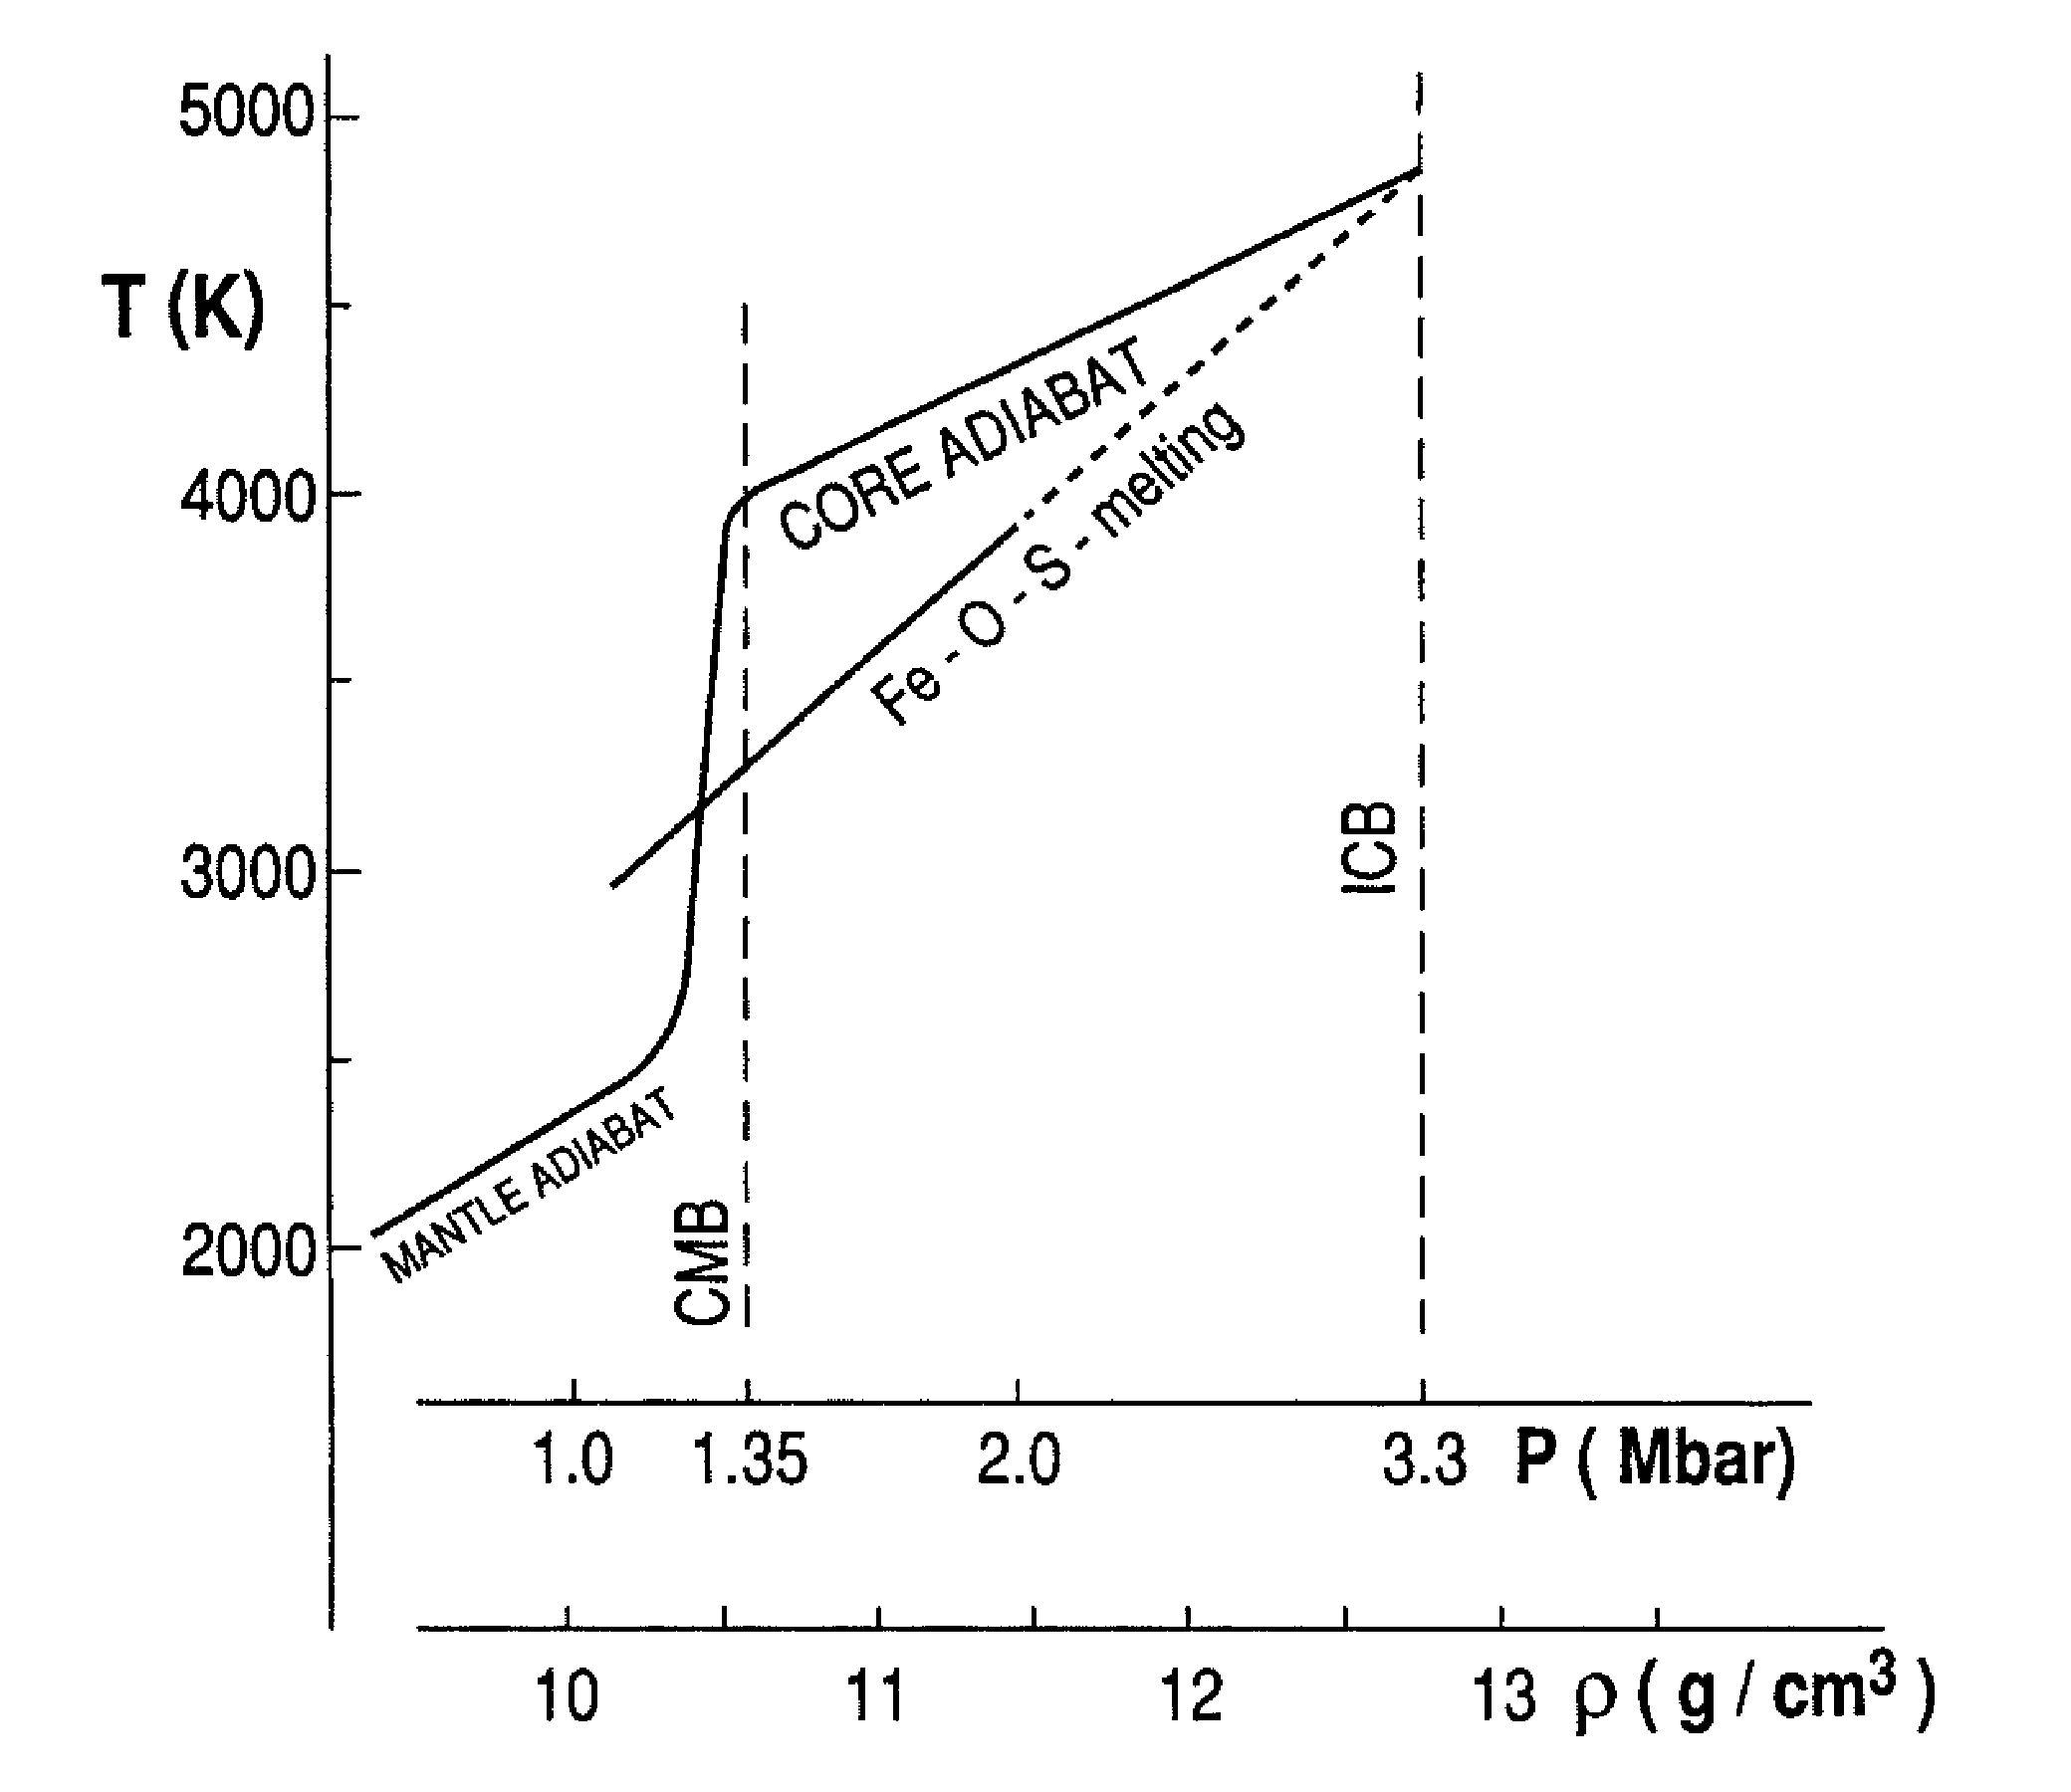
\includegraphics[width=7cm]{images/gravity/boehler_annrev96_fig6}\\
{\captionfont
Schematic radial temperature distribution in the mantle
           and core, constrained by major phase transitions (Boehler, 1996),
           (UM-upper mantle, LM lower mantle, OC outer core, IC inner core).
           The temperature of the upper/lower mantle boundary is 
           constrained by the $\gamma$-spinel to postspinel phase
           transition at 660 km depth.
           The temperature at the inner/outer core boundary at 
           5150 km depth (radius 1220 km) is constrained 
           by the melting temperature of the hypothetical
           core `Fe-O-S' alloy.
           The right hand frame shows a schematic core temperature 
           distribution (geotherm) labeled `CORE ADIABAT' in the 
           liquid outer core
           versus pressure and the melting curve (liquidus) of the core 
            `Fe-O-S' alloy.
           (CMB core-mantle boundary, ICB inner core boundary).
           The ICB is determined by the intersection of the liquidus
           and the geotherm.
           During core cooling the ICB moves outward as the inner core
           grows by crystallisation.}
%\label{Fig_boehler_annrev96_fig1-6}
\end{center}

Starting from these anchor points the temperature is then extrapolated 
from both sides to the core mantle boundary at 2900 km depth.
For this temperature extrapolation assumptions have to be made about 
the dominant heat transport mechanism and in this case it is assumed
that heat transport operates mainly through thermal convection.
This will be further investigated in later sections dealing with 
heat transport in the Earth's mantle.


\fbox{
\begin{minipage}{0.9\textwidth}
\begin{problem}
 {\small \it
   Estimate the temperature near the bottom of the mantle by adiabatic
   extrapolation of the temperature $T_{660} ~\sim~ 1900 \mathrm{K}$
   of the phase transition near 660 km depth, to the depth of the
   core mantle boundary, using the general expression for the
   adiabat in a homogeneous layer.

   Hints:
   apply the result of problem \ref{problem-WA-temperature} and
   assume uniform values of the `scale height parameter'
     $H_T = (\alpha g/c_P )^{-1}$, with
     $\alpha=2\cdot 10^{-5} \mathrm{K^{-1}}$, 
     $g=10 \mathrm{m s^{-2}}$,
     $c_P=1250 \mathrm{J kg^{-1}K^{-1}}$. 
   Further: approximate the adiabat by a linear depth function,
   in agreement with the schematic diagram of Boehler (1996) - see  
   figure above -to obtain a uniform 
   adiabatic temperature gradient.
 }
\end{problem}
\end{minipage}
}

\vspace{.5cm}

The `head' of the extrapolated outer core adiabat is at a temperature
of approximately 4000 K and the `foot' of the lower mantle adiabat at
approximately 2700 K.
This result indicates a large temperature contrast of about 1300 K
across the CMB.

How can such a large contrast be explained physically?
As we will see later, this can be explained by interpreting the CMB 
as a boundary between two separately convecting fluid layers, each with
a thermal boundary layer where the main heat transport mechanism shifts
from convection in the interior of the fluid layers, 
to conduction near the boundary interface, 
where vertical convective transport 
vanishes with the flow velocity component normal to the boundary. 
Separately convecting layers are in agreement with the large density
contrast across the CMB where the density almost doubles,
as illustrated in the PREM profile.
The resulting strong temperature contrast across the CMB is consistent 
with a lower mantle in a state of vigorous thermal convection.

\vspace{.5cm}

\fbox{
\begin{minipage}{0.9\textwidth}
\begin{problem}
 {\small \it
Explain why we can not turn this argument around and conclude
from these indications for a strong temperature contrast at CMB
that the mantle convects vigorously.

Hint: Check Appendix \ref{Appnd_adiabatic_temperature_profile}
for the assumptions made for an adiabatic geotherm
in the lower mantle.
}
\end{problem}
\end{minipage}
}

\vspace{.5cm}

More recent developments, providing independent information, shed new light 
on the temperature distribution in the bottom layer of the lower mantle.
A previously unknown mantle phase transition has been identified,
in the main constituent magnesium-perovskite, to a 
($\sim$ 1.5\%) denser phase
(post-perovskite) both in experimental HPT and theoretical 
(mineral physics) work at temperatures and pressure conditions
corresponding to a region in the lowermost mantle close to the 
core-mantle boundary.
This is illustrated in the figure hereafter 
showing experimental data points delineating the phase boundary.

\begin{center}
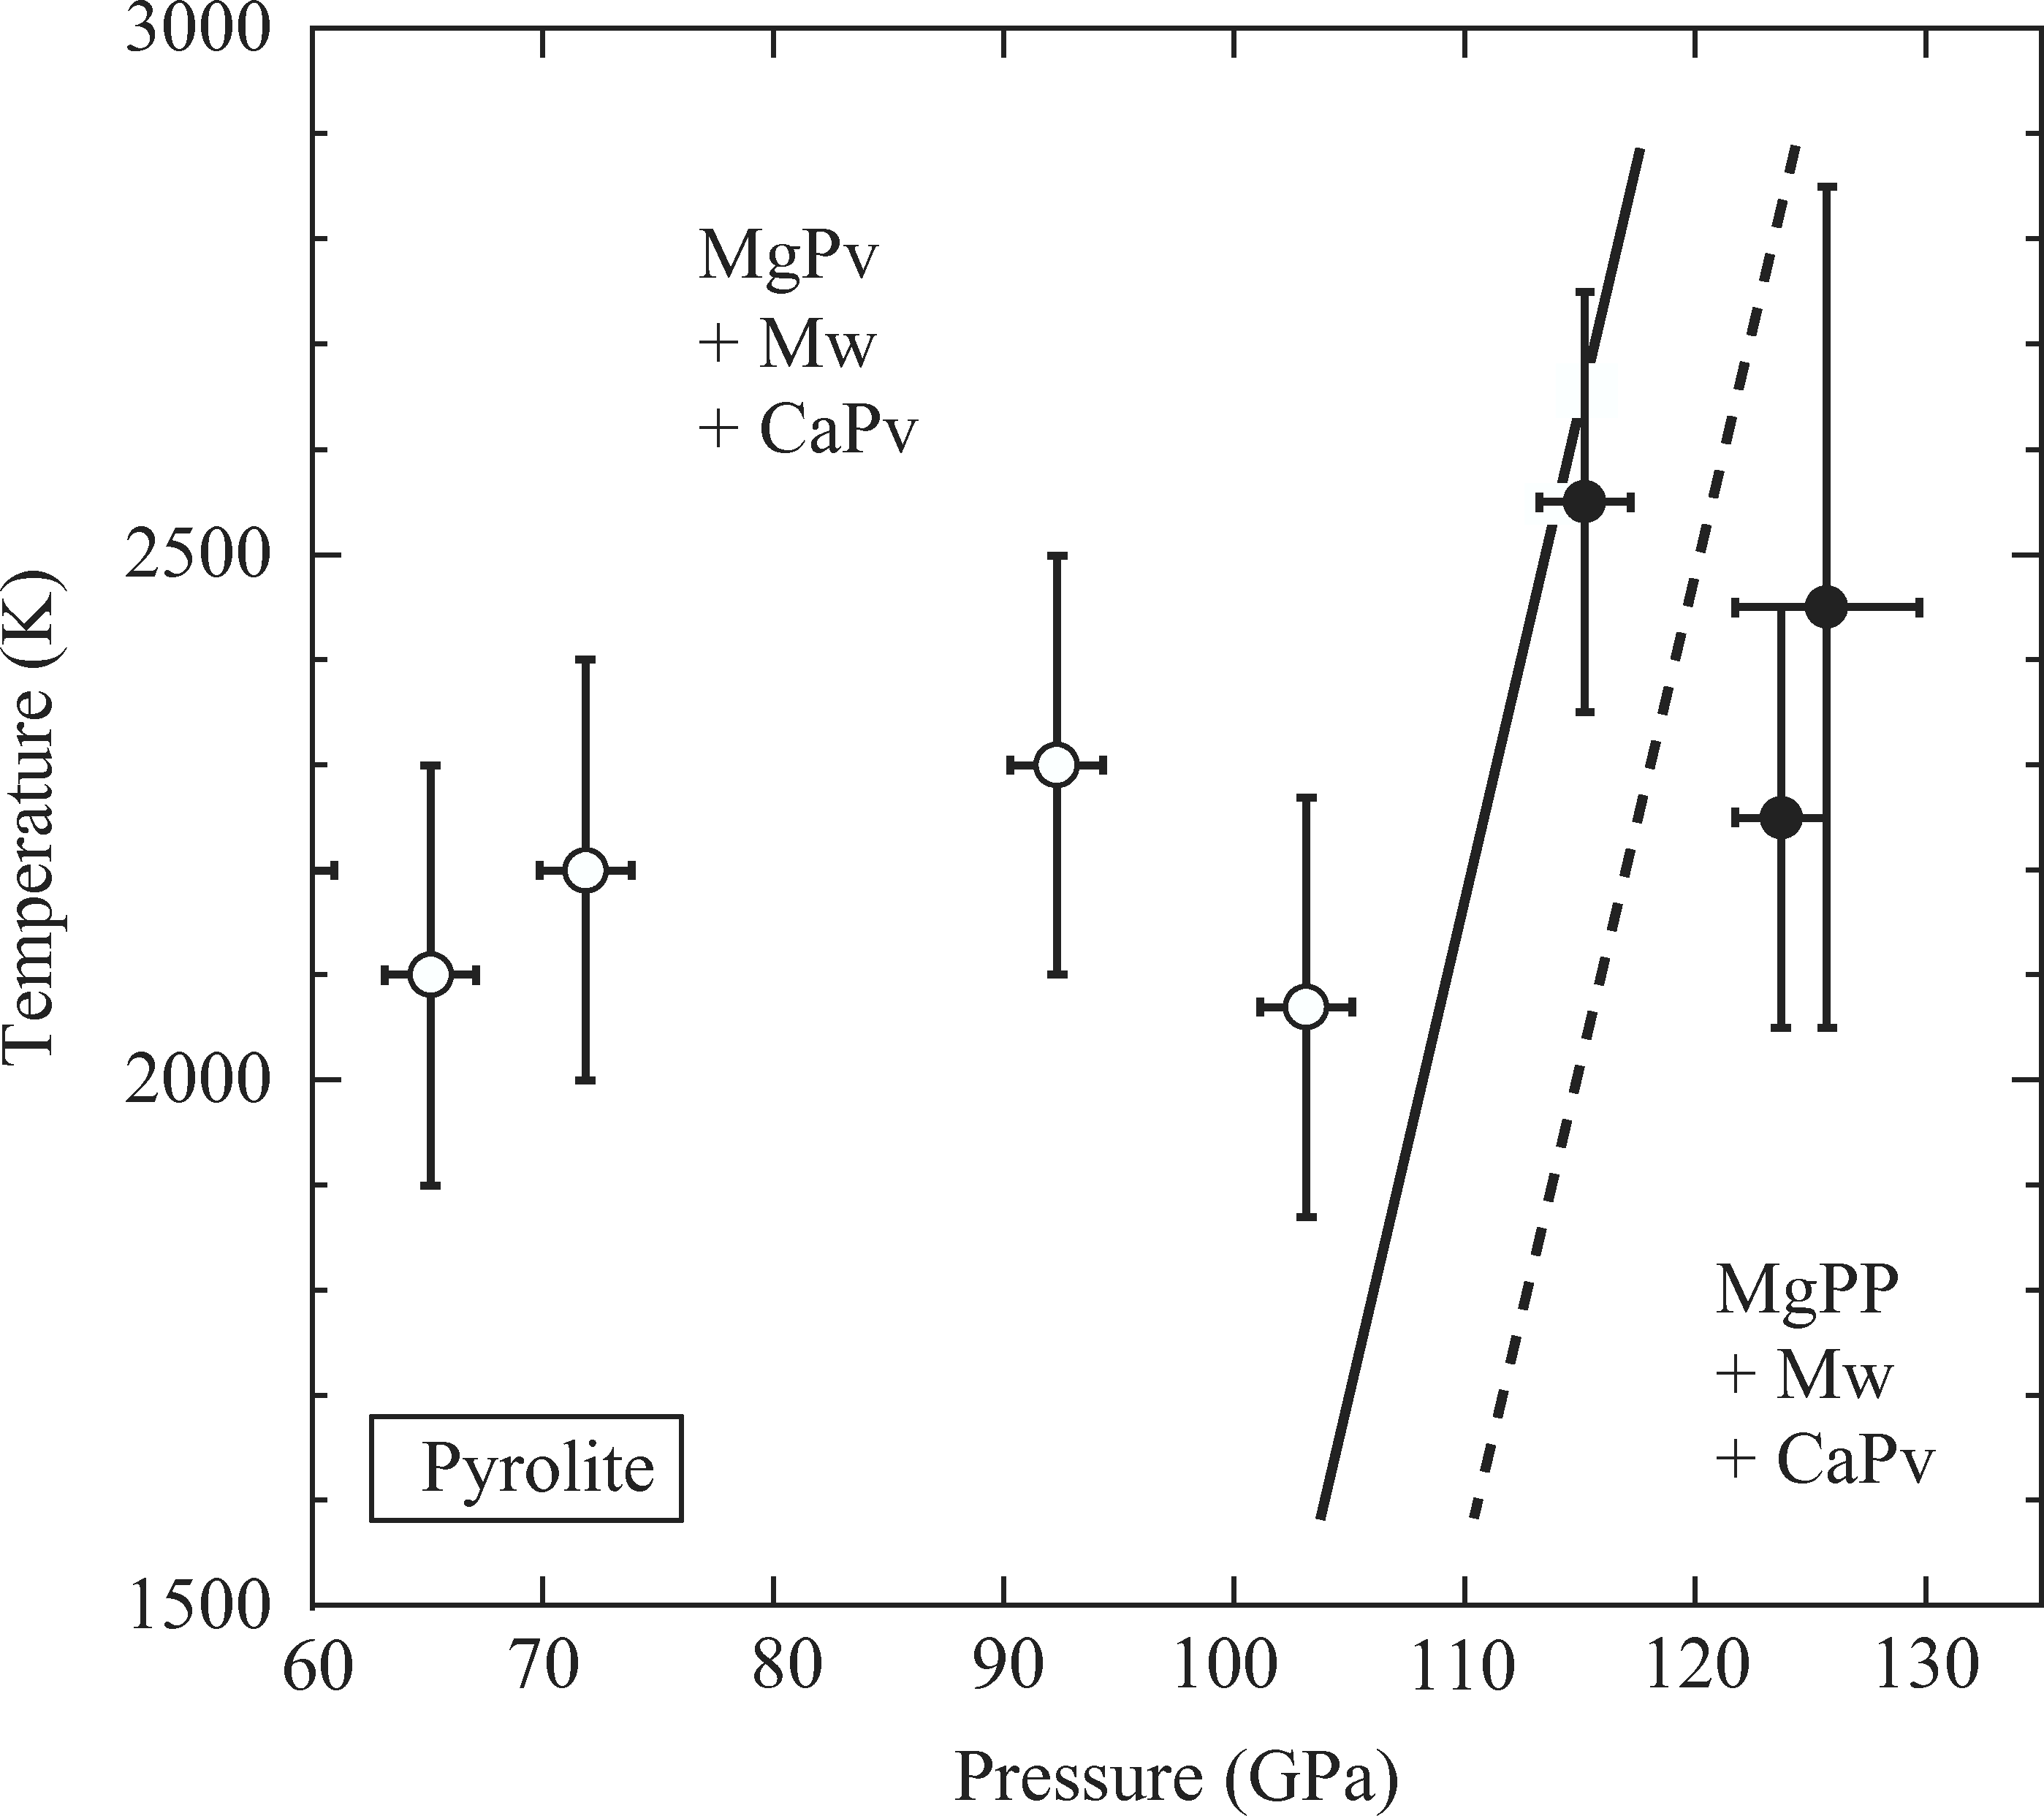
\includegraphics[width=7cm]{images/gravity/hirose_fig1}
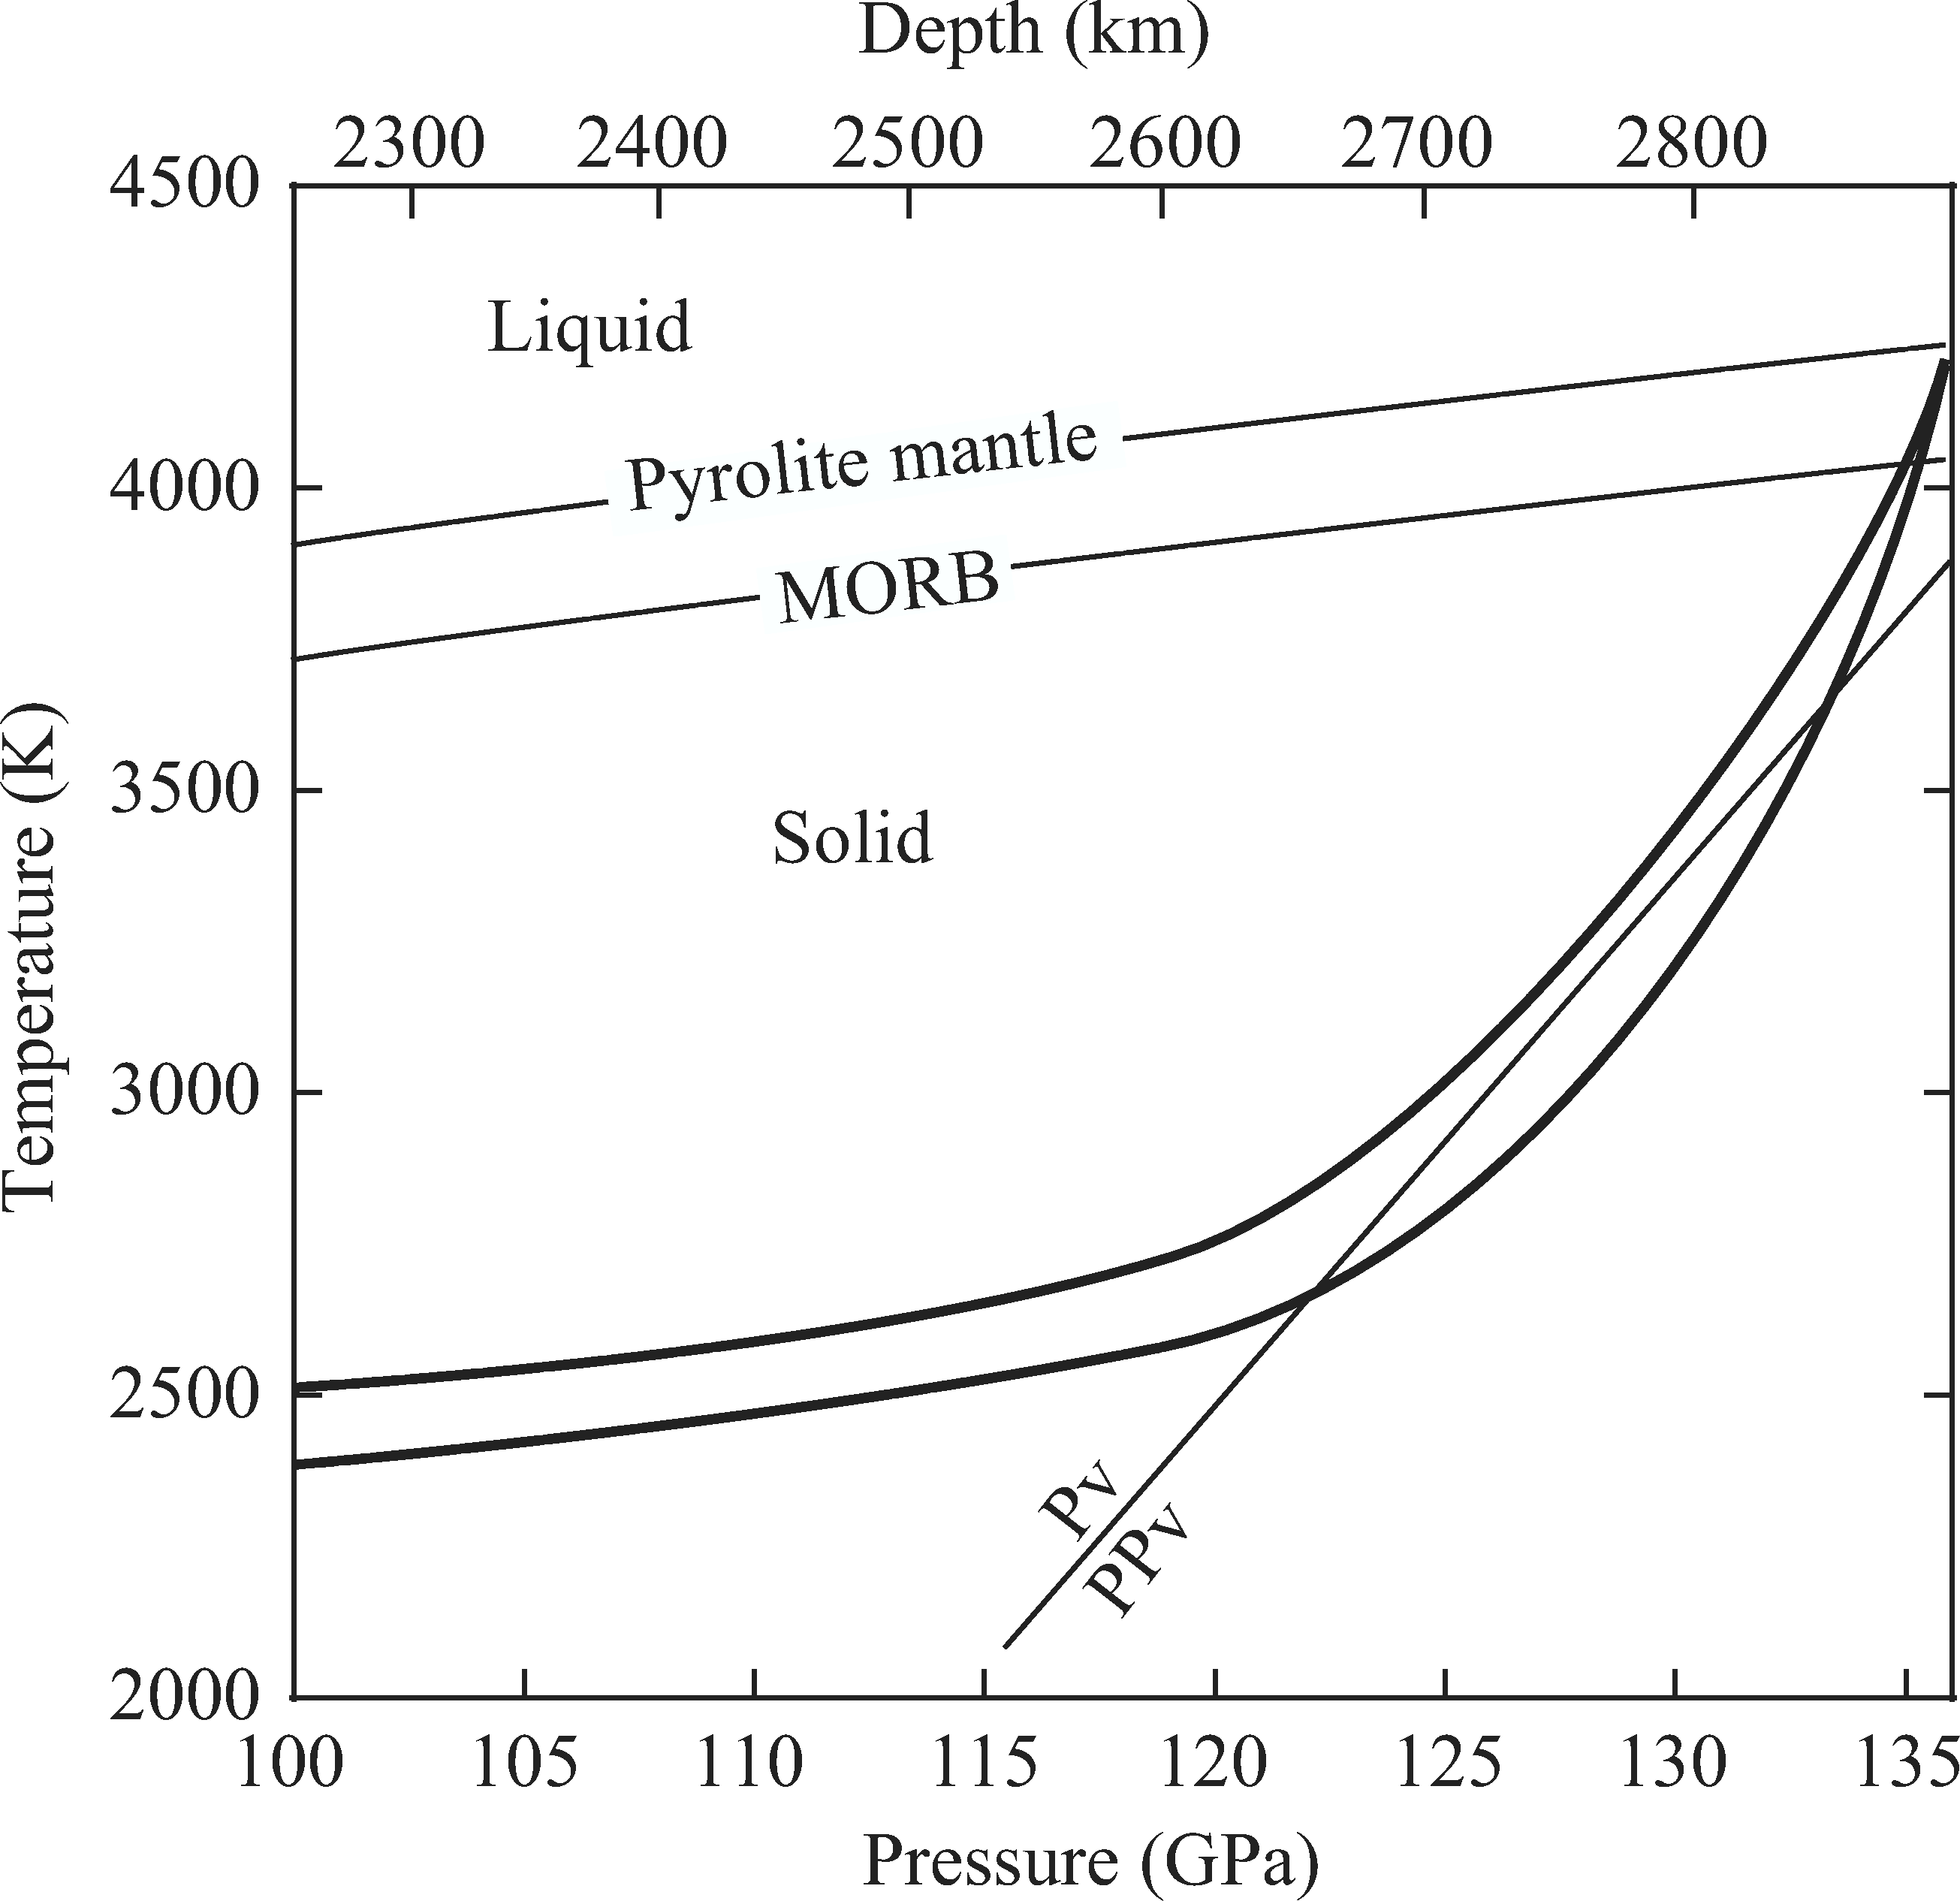
\includegraphics[width=7cm]{images/gravity/hirose_fig5}\\
{\captionfont
Left: phase relations near the bottom of the mantle for 
          pyrolitic material (Hirose, 2007).
          The solid- and dashed line correspond to different
          pressure calibration of the HPT experiments. 
          The Clapeyron slope of the phase boundary is 
          assumed $11.5 ~MPa/K$. 
          CaPv: $CaSiO_3$ perovskite
          MgPv: $MgSiO_3$-rich perovskite,
          MgPP: $MgSiO_3$-rich post-perovskite,
          Mw: magnesiow\"{u}stite.
       Right: schematic temperature profiles in the lower mantle 
       in relation to
       the perovskite (PV) to postperovskite (PPV) phase transition
       and the melting curve for pyrolitic mantle material and 
       subducted basaltic crust (MORB) (Hirose et al (2007) \cite{hibl07}).
}
%\label{Fig_hirose-fig1-5-Yuen_Book2007}
\end{center}


This phase transition has a high valued
positive slope of the phase boundary (Clapeyron parameter) 
$dP_t/dT \sim 10 ~ \mathrm{MPa K^{-1}}$. 
The intercept of the phase boundary with the core mantle boundary
at $\sim$ 136 GPa appears to be at a temperature several hundred Kelvin
below the temperature of the liquid metal outer core as illustrated in
the right part of the above figure.
As a consequence the geotherm may intersect the phase boundary 
at multiple depth's,
depending on the local mantle temperature, 
a phenomenon known as `double crossing' (Hernlund et al., 2005).
When a double crossing of the geotherm occurs, 
a thin layer exists directly bordering the core, where perovskite is the stable
phase while on top of this bottom PV layer, a postperovskite layer 
exists with a variable thickness of up to several hundred
kilometers.  

A further implication of the phase diagram illustrated in 
is that the PPV layer will be absent in hot regions where the
geotherm is completely above the PV-PPV phase boundary.
This post-perovskite phase boundary has also been associated with the 
top of the D" layer at variable height $\sim 100-300$ km above the CMB
(Lay et al., 2005).


These seismological interpretations of the postperovskite 
phase boundary have been based on limited resolution methods applying
1-D radial velocity models.
In a more recent development, techniques related to seismic wave
migration methods, used in the oil and gas exploration industry,
are applied to delineate reflecting interfaces in 2-D and 3-D models
in seismic stratigraphy of the CMB region (van der Hilst et al., 2007).
This way the spatial resolution has been brought down to about 20 km,
allowing mapping of detailed  structures in the lowermost mantle.
An important target of these high resolution seismic methods is 
the bottom interface of a postperovskite layer,
associated with the `double crossing', where mantle material 
transforms back from postperovskite into perovskite due to the steep 
increase in temperature in the bottom thermal boundary layer, 
illustrated in the figure above,
related to the temperature contrast across the CMB.

In a similar way as for the spinel-postspinel phase transition
the temperature  at the seismic interfaces can then be estimated
from the given depth(pressure) and the experimentally determined
parameters of the postperovskite phase transition.
This way a mantle adiabatic geotherm and boundary 
layer structure (error function) have been estimated with a CMB
temperature $T_{cmb}~\sim~ 4000$ K (van der Hilst et al., 2007).
The `foot' of the adiabatic mantle geotherm derived from this
lies at a temperature of approximately 2500 K.
Both the estimated CMB temperature and the foot of the adiabat
seem to confirm independent earlier findings based on adiabatic
temperature extrapolation over large depth ranges (Boehler, 1996 \cite{boeh96}). 

The temperature contrast of about 1500 K across the core-mantle
boundary resulting from these interpretations identify the
bottom of the mantle as a thermal boundary layer,
characteristic of a vigorously convecting layer where the boundary
interface has a fixed or slowly varying temperature,
as we will see in the section on heat transport in the mantle.
As such these results from mineral physics and seismology have
produced new evidence for strong mantle convective flow near the
core-mantle boundary.
